\section{Introduction}

\subsection{Background}
Given a set of data, we can use B-Splines as a form of regression. This method essentially creates a variety of piecewise polynomial functions of a given degree to better represent the data. It is often the case that we have too much data to process quickly so we turn to parallel programming to speed up the process.
\\ \\
We have created an R package in which the output of the function is the basis matrix containing the elements found via the Cox-de Boor recursion formula for each given $x$ value. \\ \\ The Cox-de Boor recursion formula is found as follows\footnote{\url{http://www.cs.mtu.edu/~shene/COURSES/cs3621/NOTES/spline/B-spline/bspline-basis.html}}:
\begin{center} 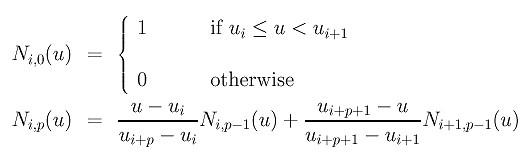
\includegraphics[scale=.6]{recursion.jpeg} \end{center}

This code could then be applied to regress as follows:
\begin{verbatim}
n <- 1000
x <- seq(0, 1, length=n)
B <- bs(x) #use default
dgp <- sin(2*pi*x)
y <- dgp + rnorm(n, sd=.1)
model <- lm(y~B-1)
plot(x, y, cex=.25, col="grey")
lines(x, fitted(model), lwd=2)
lines(x, dgp, col="red", lty=2)
\end{verbatim}

The code to the functions implemented to generate the B-Spline matrix can be viewed in the appendix for serial R, OpenMP, CUDA, and SNOW.

\subsection{Serial R} %completed
As a benchmark, we found a simplified version of the B-Spline $bs()$ function in serial R\footnote{\url{http://cran.r-project.org/web/packages/crs/vignettes/spline_primer.pdf}}.
This version heavily relies on the Cox-de Boor recursion formula to generate the B-Spline. This allowed a clear and direct method of calculating the matrix for basis splines. This function was used as the basis of parallelization; modifications were made to exploit each column of the basis matrix to speed up the process while incorporating recursion whenever possible.

%For each degree of a polynomial, a given vector of $n$ values was compared to a calculated vector of $k$ knots.

%The following recursive equation\footnote{\url{http://www.cs.mtu.edu/~shene/COURSES/cs3621/NOTES/spline/B-spline/bspline-basis.html}} was the basis for all computations:



\subsection{OpenMP} %completed
OpenMP allowed the recursive algorithm to be implemented in parallel. As shown in the
time trials, this meant significant improvement in computational time. The main set up of the
function mirrored the serial function in R with only a few minor changes. The heart of the algorithm still
existed in the Cox-de Boor recursive formula. We used an omp parallel for loop through each column oto speed up the formation of the output basis matrix. Inside the parallel loop, an omp critical section is used when storing a returned column to assure no overwriting takes place.


\subsection{CUDA} %completed
At the core, R uses data type double when dealing with real numbers. CUDA does not support the data type double, and thus, forces a conversion from type double to type float. Due to this conversion, basic memory allocation becomes unpredictable as double is composed of 8-bits as is float composed of 4-bits. This caused many irregularities while copying the arrays for x, knots, and the eventual basis matrix to and from the CUDA device.
\\ \\
The original approach was to follow a similar algorithm as in the serial R version. However, CUDA does not support recursion, and thus, the algorithm needed modification. Emulating an algorithm optimized for recursion often tends to be difficult and requires much more overhead.
\\ \\
The first approach to an iterative algorithm took use of stacks. The idea was to skip the break down and go directly into the build up. In other words, we were to start from the base case and follow the recursive algorithm in a forward manner exploiting the Cox-de Boors recursion formula in an iterative manner. For reasons unknown, this approach did not work.
\\ \\
The next approach was to follow a triangular method of computation, filling each index of the return matrix as the algorithm went forward. The Triangular method is described by the following graphic:
\begin{center} 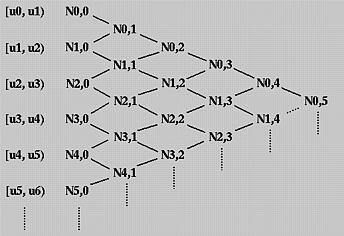
\includegraphics[scale=.6]{triangle.jpg} \end{center}
Again, this approach was unsuccessful as it a range error.
\\ \\
The final approach was to separate tasks – it would be recursive to the point of the base case. Once entering the base case, when the current degree of the polynomial was equal to zero, knot[i] and knot[i+1] were sent, along with the entire $x$ vector, to the CUDA device. Once on the device, each $x$ value was used in the calculation using parallelization and passed back to the host where it was returned to the basis matrix. Once out of the base case, for any degree greater than zero and less than the given degree, the usual recursive algorithm was used.
\\ \\
As a result, the CUDA algorithm is essentially serial with a small taste of parallel for a minimal speedup. We can still expect improvement from the CUDA algorithm as opposed to the serial version but there is still more optimization that can be done on the CUDA algorithm to make full use of the benefits of a GPU. Therefore, this isn't expected to be a match for the other parallel algorithms but it can at least acheive the job of improving computation time by a bit.


\subsection{SNOW}
SNOW also exploits the recursive algorithm to find each element in the matrix. SNOW also has the advantage of using the vectorization style that the R programming language has been optimized for, which can give better computational times. The main setup of the function mirrors the serial function in R with each cluster working on a different column of the final output matrix. It gives the worker clusters all the necessary information and then has them find the elements of the particular column they were assigned to. The code gives the user the option to select how many clusters to use and the code is designed to automatically make the clusters for the user.
